\section{Results}\label{sec:results}
\mr{TODO: The mean density and cross power spectrum $\chi^{2}$ diagnostics do not reveal any signature of remaining systematic effects -- given all the available templates. But we could be missing some unknown maps. There are some calibration maps made by Aaron which I need to look into. I did not use the Gaia stellar map for training-- Zhou et al has a discussion on why it should not be used. But I plan to apply some cuts based on imaging (e.g., poor depth, high stellar density and extinction) to see if those impact the best fit estimates. Next, I will study how changing the lowest ell used could affect our results. }

\subsection{Lognormal Mocks}

Corner plots of the PNG parameter $\fnl$ and bias coefficient are shown in Fig. \ref{fig:mcmc_mocks} for fitting the mean power spectrum of the mocks, with and without $\fnl$. Maximum-A-Posteriori estimates and marginalized mean, median and $1\sigma$ quantiles are summarized in Tab. \ref{tab:mocksmcmc}. Comparing DECaLS North with sky coverage $0.14$ to full DESI with $0.40$, we find the constraint improve by a factor of $1.9$ which is slightly more than $\sim f_{\rm SKY}^{-1/2}$, 1.7. while As a robustness test, we also fit the mean power spectrum of the $\fnl=100$ mocks using the covariance matrix estimated from the $\fnl=0$ mocks. We find that the constraints improve by a factor of $4.2$, due to a higher signal to noise ratio.

\begin{table*}
  \begin{center}
    \caption{Maximum-A-Posteriori (MAP) and marginalized mean estimates for $\fnl$ from fitting the mean power spectrum of the mocks. Degree of freedom is 33 (37 data points - 3 parameters - 1).}
    \label{tab:mocksmcmc}
    \begin{tabular}{lllccccc}
    \hline
    \hline
Mock $\fnl$ &  Footprint   &  Observable & 	Best fit  & Mean & $ 68\%$ CL & $ 95\%$ CL & $\chi^{2}$ \\
    \hline
$\fnl=100$ & DESI & log$C_{\ell}$                           & $100.97$& $100.97$& $100.33<\fnl<101.61$& $ 99.72<\fnl<102.23$ &   38.8\\
$\fnl=100$ & DESI & $C_{\ell}$                              & $100.97$& $100.95$& $100.32<\fnl<101.58$& $ 99.71<\fnl<102.18$ &   39.0\\
$\fnl=100$ & DESI & log$C_{\ell}$ using $f_{\rm NL}=0$ cov  & $101.01$& $101.03$& $100.42<\fnl<101.63$& $ 99.85<\fnl<102.21$ &   39.9\\
$\fnl=100$ & DESI & $C_{\ell}$ using $f_{\rm NL}=0$ cov     & $100.13$& $100.13$& $100.00<\fnl<100.26$& $ 99.88<\fnl<100.38$ &  207.6\\
\hline
$\fnl=0$ &DESI      &        log$C_{\ell}$                  & $  0.47$& $  0.47$& $  0.08<\fnl<  0.85$& $ -0.30<\fnl<  1.22$ &   35.7\\
$\fnl=0$ & DECaLS North &         log$C_{\ell}$               & $  0.09$& $  0.08$& $ -0.61<\fnl<  0.78$& $ -1.29<\fnl<  1.45$ &   26.7\\
$\fnl=0$ & DECaLS South  &                     log$C_{\ell}$ & $  0.87$& $  0.88$& $  0.16<\fnl<  1.58$& $ -0.52<\fnl<  2.27$ &   34.3\\
$\fnl=0$ & BASS+MzLS  &  log$C_{\ell}$                       & $  1.07$& $  1.07$& $  0.32<\fnl<  1.82$& $ -0.40<\fnl<  2.55$ &   39.4\\ 
\hline
    \end{tabular}
  \end{center}
\end{table*}


\begin{figure*}
    \centering
    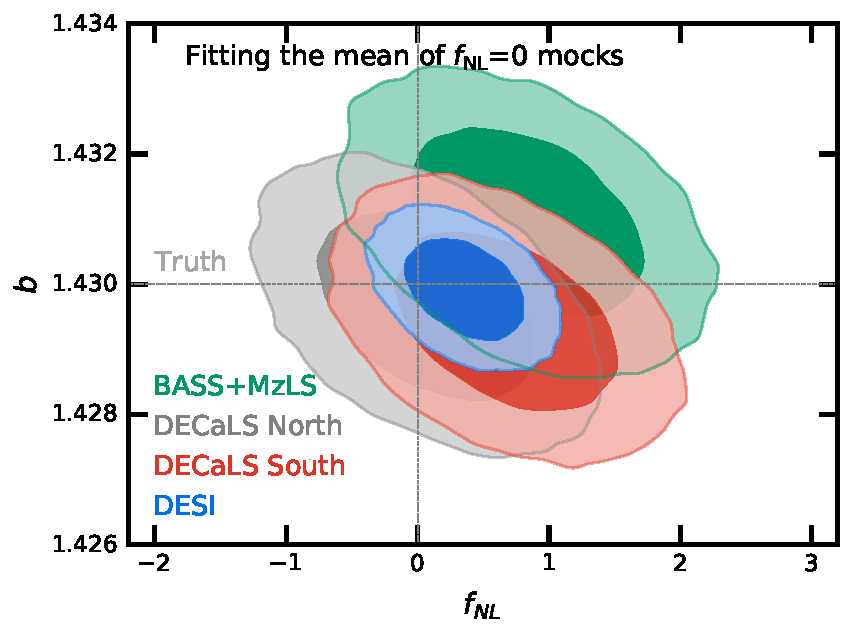
\includegraphics[width=0.45\textwidth]{figures/mcmc_zero.pdf} 
    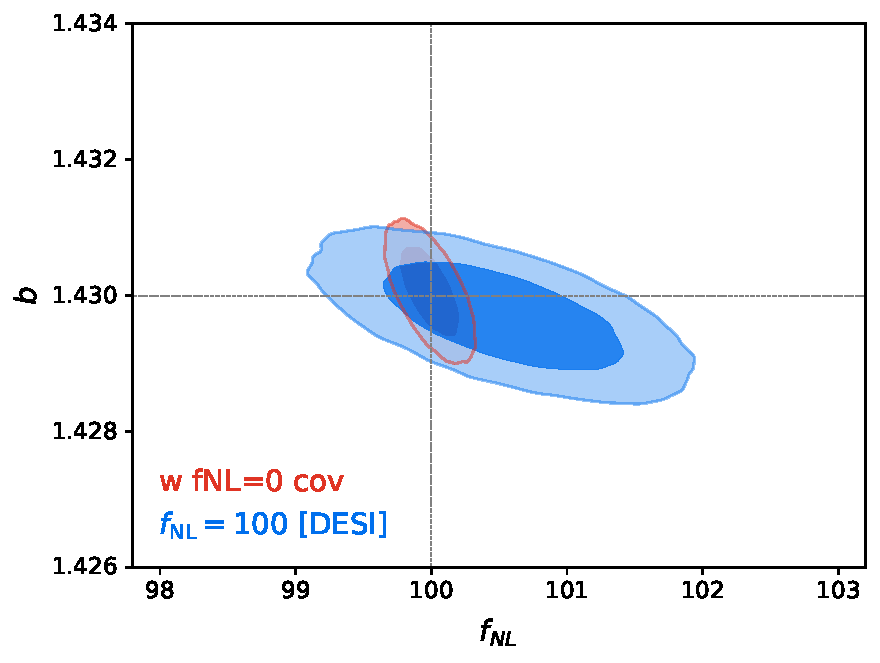
\includegraphics[width=0.45\textwidth]{figures/mcmc_po100.pdf} 
    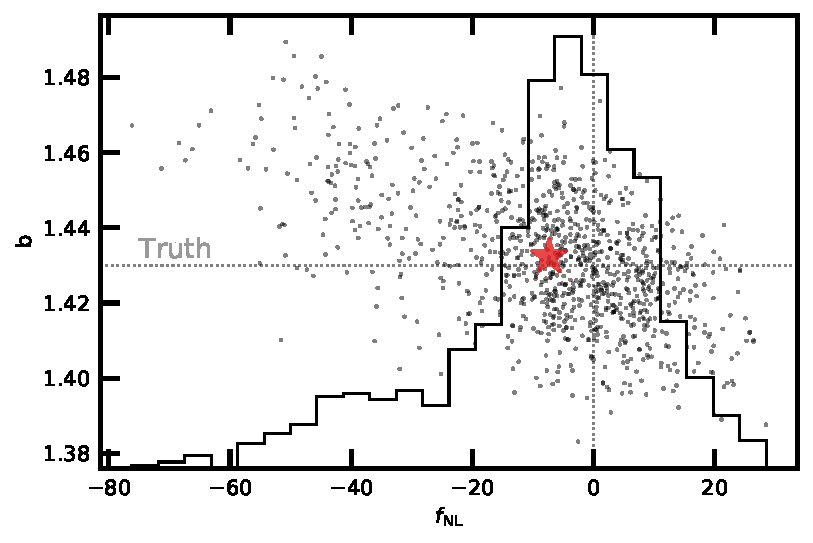
\includegraphics[width=0.45\textwidth]{figures/bestfit_zero.pdf} 
    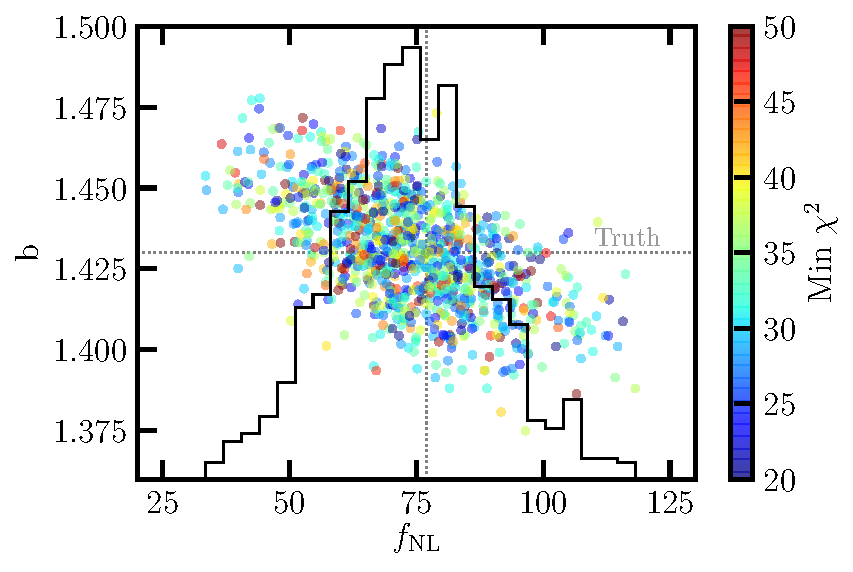
\includegraphics[width=0.45\textwidth]{figures/bestfit_po100.pdf}         
    \caption{Top: 68\% and 95\% confidence contours for $\fnl=0$ (left) and $100$ (right) mocks. Using the $\log C_{\ell}$ fitting yield constraints that are insensitive to the covariance used. Bottom: best fit estimates from fitting 1000 lognormal mocks with $\fnl=0$ (left) and $100$ (right) in the DESI footprint. The truth values are represented by vertical and horizontal lines, and the mean of best fit estimates are denoted by the red stars.}\label{fig:mcmc_mocks}
\end{figure*}



\subsection{DR9 LRGs}
\begin{table*}
  \begin{center}
    \caption{Maximum-A-Posteriori (MAP) and marginalized mean estimates for $\fnl$ from fitting power spectrum of DR9 LRGs for DESI footprint before and after correcting for systematics. Degree of freedom is 33 (37 data points - 3 parameters - 1).}
    \label{tab:dr9method}
    \begin{tabular}{llccccc}
    \hline
    \hline
Footprint   & Method & 	Best fit  & Mean & $ 68\%$ CL & $ 95\%$ CL & $\chi^{2}$ \\
    \hline
DESI & No Weight                               & $147.13$& $150.13$& $127.58<\fnl<172.76$& $108.56<\fnl<197.07$ &   44.4\\
DESI &Linear (all maps)                                & $ 46.87$& $ 49.04$& $ 33.97<\fnl< 63.98$& $ 21.21<\fnl< 81.00$ &   41.1\\
DESI &Linear (Conservative I)                          & $ 64.46$& $ 66.69$& $ 49.67<\fnl< 83.63$& $ 35.64<\fnl<102.59$ &   38.8\\
DESI &Linear (Conservative II)                         & $ 47.62$& $ 49.54$& $ 34.21<\fnl< 64.81$& $ 21.27<\fnl< 82.06$ &   39.6\\
DESI & Nonlinear (Conservative II)                    & $ 37.15$& $ 38.73$& $ 24.58<\fnl< 52.77$& $ 12.32<\fnl< 68.55$ &   34.6\\
\hline
BASS+MzLS & Nonlinear (Cons. II)          & $ 20.06$& $ 24.71$& $ -1.52<\fnl< 51.26$& $-24.95<\fnl< 82.62$ &   35.6\\
DECaLS North    & Nonlinear (Cons. II)                               & $ 53.33$& $ 58.36$& $ 30.33<\fnl< 86.81$& $  6.45<\fnl<120.93$ &   41.1\\
DECaLS North   & Nonlinear (Cons. II+CALIBZ+logHI)             & $ 72.10$& $ 78.57$& $ 47.81<\fnl<109.27$& $ 23.22<\fnl<146.65$ &   38.4\\
DECaLS North [incl. DEC $< -11$] & Nonlinear (Cons. II)                & $ 53.36$& $ 58.27$& $ 30.65<\fnl< 85.91$& $  8.33<\fnl<118.84$ &   40.7\\
DECaLS South    & Nonlinear (Cons. II)                               & $ 40.61$& $ 43.17$& $ 19.36<\fnl< 68.11$& $ -6.64<\fnl< 96.65$ &   30.2\\
DECaLS South & Nonlinear (Cons. II+CALIBZ+logHI)            & $ 43.93$& $ 48.74$& $ 23.02<\fnl< 74.64$& $ -0.40<\fnl<105.22$ &   30.8\\
DECaLS South [incl. DEC $< -30$] & Nonlinear (Cons. II)                & $ 56.93$& $ 60.83$& $ 39.20<\fnl< 82.44$& $ 21.30<\fnl<107.53$ &   23.8\\
%
%
%
%
%    
%DESI & No Weight                               & $147.13$& $150.13$& $127.58<\fnl<172.76$& $108.56<\fnl<197.07$\\
%\hline
%DESI &Linear (all maps)                                & $ 46.87$& $ 49.04$& $ 33.97<\fnl< 63.98$& $ 21.21<\fnl< 81.00$\\
%DESI &Linear (Conservative I)                          & $ 64.46$& $ 66.69$& $ 49.67<\fnl< 83.63$& $ 35.64<\fnl<102.59$\\
%DESI &Linear (Conservative II)                         & $ 47.62$& $ 49.54$& $ 34.21<\fnl< 64.81$& $ 21.27<\fnl< 82.06$\\
%DESI &Nonlinear (Conservative II)                    & $ 37.15$& $ 38.73$& $ 24.58<\fnl< 52.77$& $ 12.32<\fnl< 68.55$\\
%\hline
%BASS+MzLS & Nonlinear (Cons. II)    & $ 20.06$& $ 24.71$& $ -1.52<\fnl< 51.26$& $-24.95<\fnl< 82.62$\\
%DECaLS North    &Nonlinear (Cons. II)                        & $ 53.33$& $ 58.36$& $ 30.33<\fnl< 86.81$& $  6.45<\fnl<120.93$\\
%DECaLS North & Nonlinear (Cons. II+CALIBZ+logHI)     & $ 72.10$& $ 78.57$& $ 47.81<\fnl<109.27$& $ 23.22<\fnl<146.65$\\
%DECaLS North [incl. DEC $< -11$]   &Nonlinear (Cons. II)       & $ 53.36$& $ 58.27$& $ 30.65<\fnl< 85.91$& $  8.33<\fnl<118.84$\\
%DECaLS South      &Nonlinear (Cons. II)                        & $ 40.61$& $ 43.17$& $ 19.36<\fnl< 68.11$& $ -6.64<\fnl< 96.65$\\
%DECaLS South & Nonlinear (Cons. II+CALIBZ+logHI)       & $ 43.93$& $ 48.74$& $ 23.02<\fnl< 74.64$& $ -0.40<\fnl<105.22$\\
%DECaLS South [incl. DEC $ < -30$]  &Nonlinear (Cons. II)          & $ 56.93$& $ 60.83$& $ 39.20<\fnl< 82.44$& $ 21.30<\fnl<107.53$\\
    \end{tabular}
  \end{center}
\end{table*}


\begin{figure*}
    \centering
    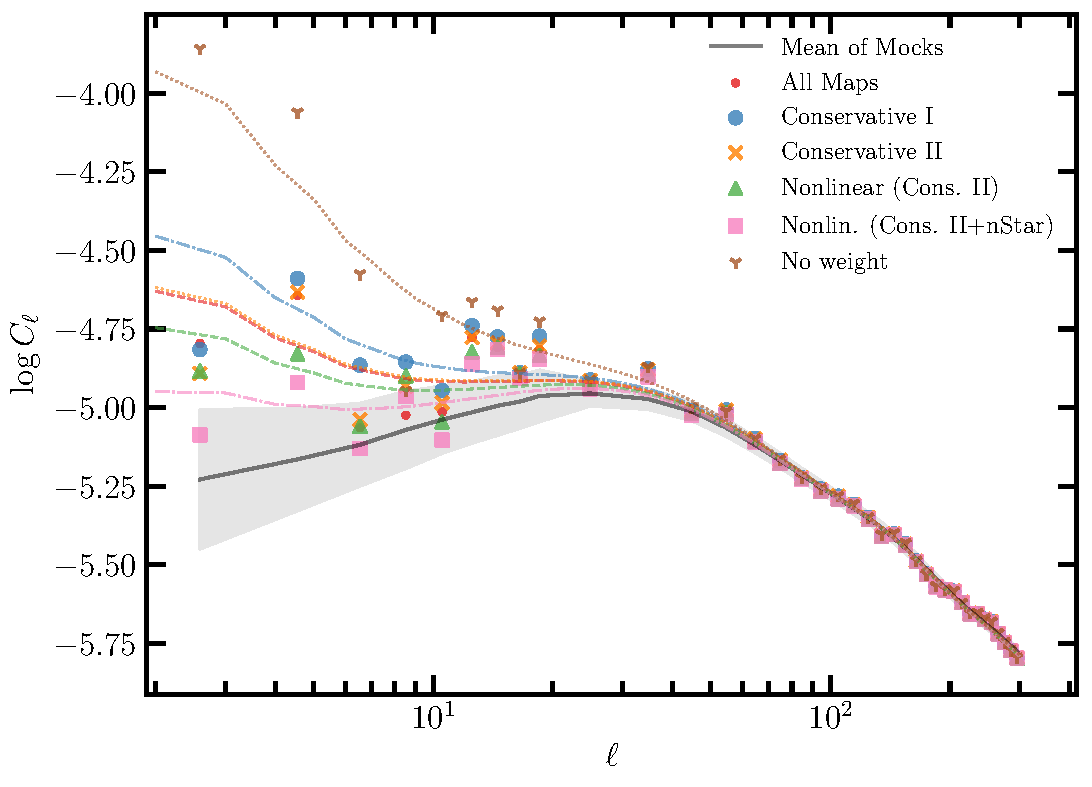
\includegraphics[width=0.95\textwidth]{figures/model_dr9.pdf} 
    \caption{Measured power spectrum of the DR9 LRG sample before and after correcting for systematics with their corresponding best fit theory predictions. The shade represents $1\sigma$ error constructed from the $\fnl=0$ mocks.}
    \label{fig:cl_dr9}
\end{figure*}

\begin{figure*}
\centering
    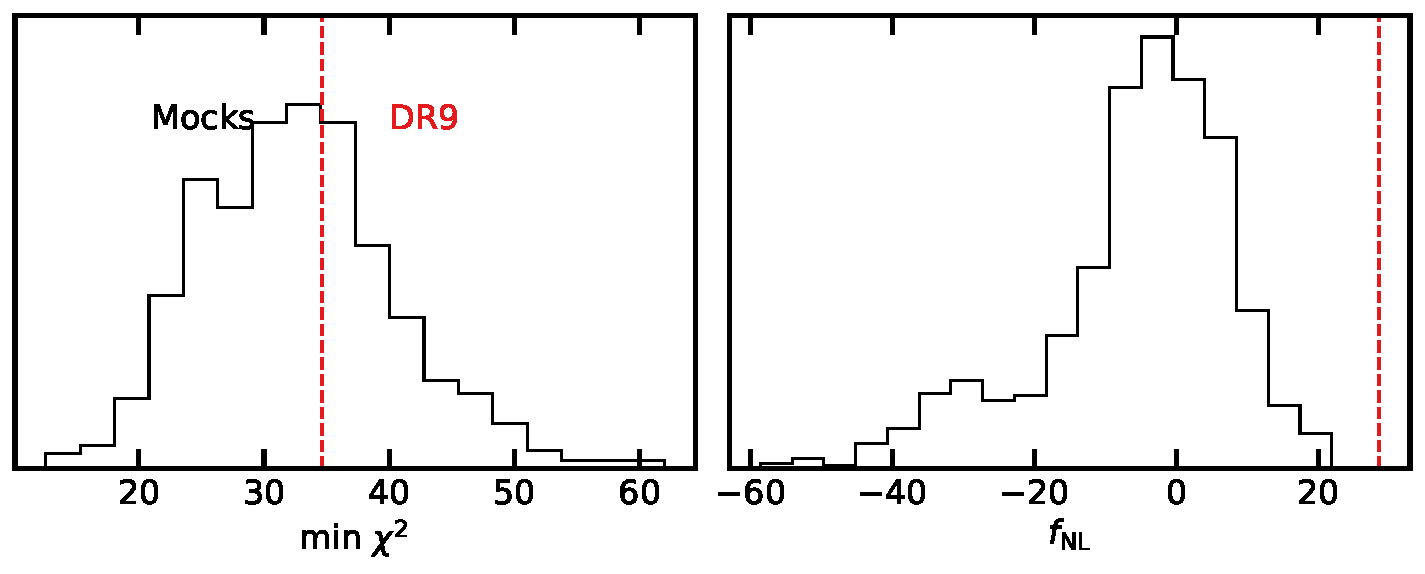
\includegraphics[width=0.95\textwidth]{figures/pdf_dr9vsmocks.pdf} 
    \caption{}\label{fig:dr9vsmocks}
\end{figure*}

\begin{figure*}
    \centering
    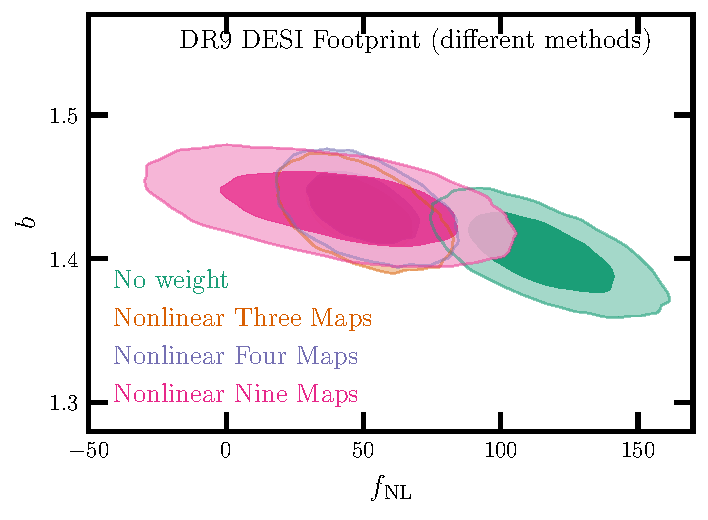
\includegraphics[width=0.95\textwidth]{figures/mcmc_dr9methods.pdf} 
    \caption{DR9 LRGs for DESI footprint.}\label{fig:mcmc_dr9}
\end{figure*}

\begin{figure*}
    \centering
    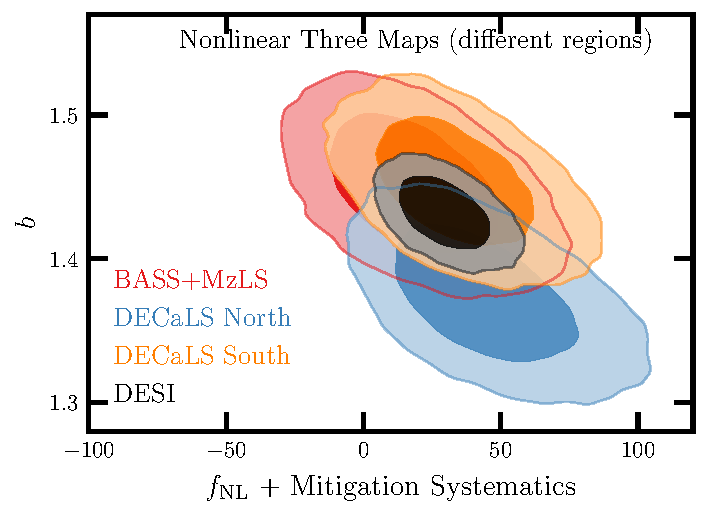
\includegraphics[width=0.95\textwidth]{figures/mcmc_dr9regions.pdf} 
    \caption{DR9 LRGs for each individual imaging survey.}\label{fig:mcmc_dr9reg}
\end{figure*}

\begin{figure}
    \centering
    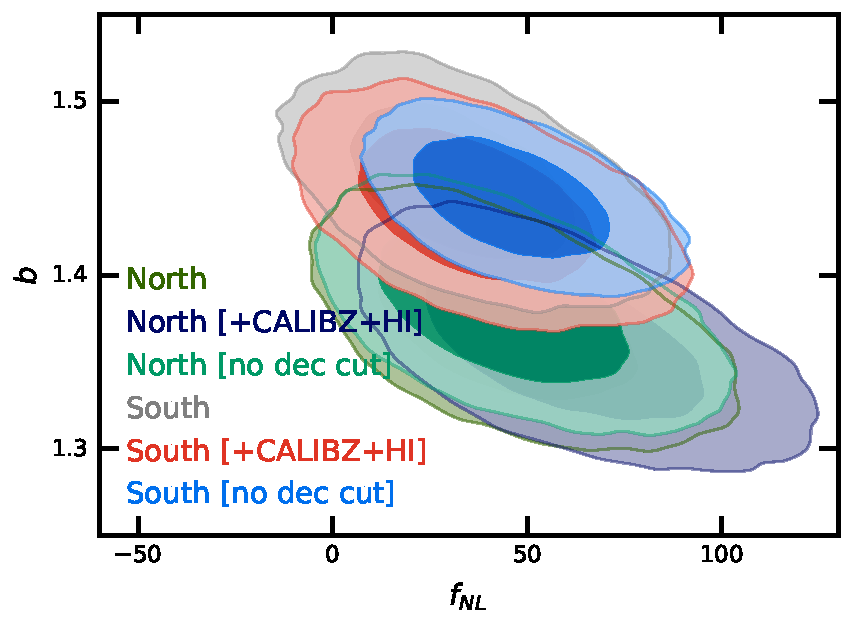
\includegraphics[width=0.45\textwidth]{figures/mcmc_dr9_cutdec.pdf}     
    \caption{Impact of cutting out spurious islands in DECaLS North and DEC < -30 in DECaLS South.}\label{fig:mcmc_dr9cuts}
\end{figure}
